\vspace{0.5cm}
\section{Implementazione e Query}

Per analizzare concretamente l'organizzazione dell’architettura del database, è stato realizzato un file SQL denominato \textbf{Concessionaria.sql}, contenente tutte le definizioni necessarie alla creazione e al popolamento delle tabelle.

Inoltre, sono stati implementati due trigger per il controllo dei dati relativi alle date e al numero progressivo, entrambi associati all’entità \textbf{Intervento}.

Per comprendere il comportamento del database durante il suo ciclo di vita, sono state sviluppate cinque query di esempio finalizzate a verificarne il corretto funzionamento. Il file include tali query e contiene anche un indice creato appositamente per ottimizzare le prestazioni di una di esse.

\subsection{Definizione delle Query}
In questa sezione vengono presentate, una alla volta, le query selezionate, accompagnate dalle rispettive descrizioni e dai relativi output.

\begin{itemize}
    \item \textbf{Query 1:} Determinare il modello di veicolo (cioè la coppia Denominazione Commerciale e Codice Telaio) che risulta essere stato acquistato il maggior numero di volte all'interno del concessionario.
    Per l’implementazione si è scelto di utilizzare una view di supporto.
    \vspace{0.1cm}
    \begin{lstlisting}[framesep=15pt]
-- View --
CREATE VIEW VenditePerModello AS
SELECT 
    M.Denominazione_Commerciale, 
    M.Codice_Telaio,
    COUNT(*) AS Numero_Vendite
FROM MODELLO M
JOIN VEICOLO V ON M.Denominazione_Commerciale = V.Denominazione_Commerciale 
               AND M.Codice_Telaio = V.Codice_Telaio
JOIN ACQUISTO A ON V.VIN = A.Veicolo
GROUP BY M.Denominazione_Commerciale, M.Codice_Telaio;
        
-- Query --
SELECT *
FROM VenditePerModello
WHERE Numero_Vendite = (SELECT MAX(Numero_Vendite) FROM VenditePerModello);
    \end{lstlisting}
    \begin{center}
        \textbf{OUTPUT}
    \end{center}
    
    \begin{figure}[H]
    \begin{adjustwidth}{-1cm}{-2cm}
        \centering
        
        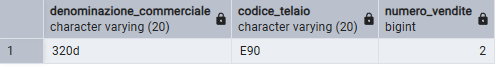
\includegraphics[keepaspectratio]{allegati/Query1.png}
        \end{adjustwidth}
    \end{figure}

    \vspace{0.2cm}
    \item \textbf{Query 2:} Selezionare i venditori che, in un intervallo temporale scelto dall'utente, hanno effettuato un numero di vendite superiore a una soglia minima fornita a runtime.
    \newline La query restituisce il codice matricola, il nome, il cognome del venditore e il conteggio delle vendite nel periodo.
    
    \vspace{0.1cm}
    \begin{lstlisting}[framesep=15pt]
SELECT D.Matricola, D.Nome, D.Cognome, COUNT(*) AS vendite
FROM VENDITORE V
JOIN DIPENDENTE D ON V.Matricola = D.Matricola
JOIN ACQUISTO A ON V.Matricola = A.Venditore
WHERE A.Data_Acquisto BETWEEN $1 AND $2   -- $1,$2 = Data Inizio/Fine
GROUP BY D.Matricola, D.Nome, D.Cognome
HAVING COUNT(*) > $3;                     -- $3 = Soglia minima
    \end{lstlisting}
    \begin{center}
        \textbf{OUTPUT}
    \end{center}
    
    \begin{figure}[H]
    \begin{adjustwidth}{-1cm}{-2cm}
        \centering
        
        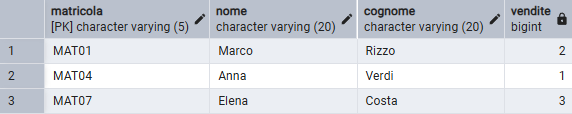
\includegraphics[keepaspectratio]{allegati/Query2.png}
        \end{adjustwidth}
    \end{figure}
    
    \vspace{0.1cm}
    \item \textbf{Query 3:} Per ciascun motore (identificato dal suo codice), determinare il ricambio che è stato utilizzato con maggiore frequenza complessiva in tutti gli interventi effettuati sui veicoli che montano quel motore. I risultati sono ordinati in senso decrescente rispetto alla quantità totale di quel ricambio utilizzata.

    \vspace{0.1cm}
    \begin{lstlisting}[framesep=15pt]
SELECT DISTINCT ON (M.Codice_Motore)
    M.Codice_Motore,
    R.OEM,
    R.Nome AS Nome_Ricambio,
    SUM(U.Quantita) AS Quantita_Totale
FROM MOTORE M

JOIN MOTORIZZATO_DA MD ON M.Codice_Motore = MD.Motore
JOIN MODELLO MO 
        ON MD.Denominazione_Commerciale = MO.Denominazione_Commerciale
        AND MD.Codice_Telaio = MO.Codice_Telaio
JOIN VEICOLO V 
        ON MO.Denominazione_Commerciale = V.Denominazione_Commerciale
        AND MO.Codice_Telaio = V.Codice_Telaio
JOIN INTERVENTO I ON V.VIN = I.Veicolo
JOIN UTILIZZA U 
        ON I.Veicolo = U.Veicolo
        AND I.Numero_Intervento = U.Numero_Intervento
JOIN RICAMBIO R ON U.Ricambio = R.OEM

GROUP BY M.Codice_Motore, R.OEM, R.Nome
ORDER BY M.Codice_Motore, Quantita_Totale DESC;
    \end{lstlisting}
    \begin{center}
        \textbf{OUTPUT}
    \end{center}
    
    \begin{figure}[H]
    \begin{adjustwidth}{-1cm}{-2cm}
        \centering
        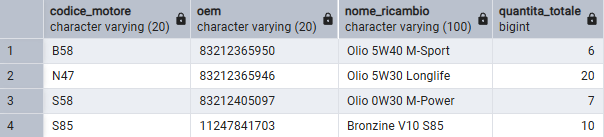
\includegraphics[keepaspectratio]{allegati/Query3.png}
        \end{adjustwidth}
    \end{figure}

    \vspace{0.1cm}
    \item \textbf{Query 4:} Per ogni possibile combinazione di frazionamento e alimentazione, calcolare il numero totale di veicoli venduti che montano un motore con quelle caratteristiche. I risultati sono ordinati in modo decrescente rispetto al numero di vendite, evidenziando le combinazioni di maggior successo commerciale. 

    \vspace{0.1cm}
    \begin{lstlisting}[framesep=15pt]
SELECT 
    M.Frazionamento,
    M.Alimentazione,
    COUNT(*) AS Numero_Vendite
FROM MOTORE M
JOIN MOTORIZZATO_DA MD ON M.Codice_Motore = MD.Motore
JOIN MODELLO MO 
        ON MD.Denominazione_Commerciale = MO.Denominazione_Commerciale 
        AND MD.Codice_Telaio = MO.Codice_Telaio
JOIN VEICOLO V 
        ON MO.Denominazione_Commerciale = V.Denominazione_Commerciale 
        AND MO.Codice_Telaio = V.Codice_Telaio
JOIN ACQUISTO A ON V.VIN = A.Veicolo

GROUP BY M.Frazionamento, M.Alimentazione
ORDER BY Numero_Vendite DESC;
    \end{lstlisting}
    \begin{center}
        \textbf{OUTPUT}
    \end{center}
    
    \begin{figure}[H]
    \begin{adjustwidth}{-1cm}{-2cm}
        \centering
        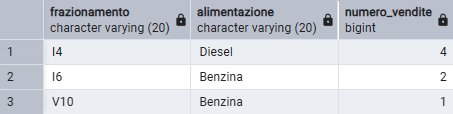
\includegraphics[keepaspectratio]{allegati/Query4.png}
        \end{adjustwidth}
    \end{figure}

    \vspace{0.1cm}
    \item \textbf{Query 5:} Calcolare il prezzo medio di vendita dei veicoli che montano un motore la cui potenza supera i 250 cv, soglia dopo cui si applica il cosiddetto “superbollo”. La query restituisce un singolo valore numerico: la media aritmetica dei prezzi degli acquisti di tali veicoli.

    \vspace{0.1cm}
    \begin{lstlisting}[framesep=15pt]
SELECT AVG(A.Prezzo) AS Prezzo_Medio_Superbollo
FROM MOTORIZZATO_DA MD
JOIN MODELLO MO 
        ON MD.Denominazione_Commerciale = MO.Denominazione_Commerciale 
        AND MD.Codice_Telaio = MO.Codice_Telaio
JOIN VEICOLO V 
        ON MO.Denominazione_Commerciale = V.Denominazione_Commerciale 
        AND MO.Codice_Telaio = V.Codice_Telaio
JOIN ACQUISTO A ON V.VIN = A.Veicolo
WHERE MD.Potenza > 250;
    \end{lstlisting}
    \begin{center}
        \textbf{OUTPUT}
    \end{center}
    
    \begin{figure}[H]
    \begin{adjustwidth}{-1cm}{-2cm}
        \centering
        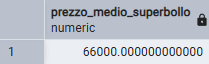
\includegraphics[keepaspectratio]{allegati/Query5.png}
        \end{adjustwidth}
    \end{figure}
\end{itemize}

\vspace{0.5cm}
\subsection{Indici}
Per migliorare le prestazioni delle interrogazioni, in particolare della query parametrica \textbf{N. 2} che richiede il filtro su un intervallo di date e il successivo raggruppamento per venditore, si è valutata l'opportunità di creare un indice sulla tabella ACQUISTO.

Essa prevede:
\begin{itemize}
    \item Un filtro su Data\_Acquisto (Per selezionare un periodo);
    \item Un GROUP BY su Venditore (Tramite la colonna Venditore che referenzia VENDITORE.Matricola);
    \item Una condizione aggregata HAVING.
\end{itemize}

\vspace{0.5cm}
\begin{lstlisting}[framesep=10pt]
CREATE INDEX idx_acquisto_data_venditore ON ACQUISTO(Data_Acquisto, Venditore);
\end{lstlisting}

\textbf{Motivazioni:}

L'indice è un \textbf{B‑Tree}, e supporta quindi le ricerche per intervallo (BETWEEN), a differenza degli hash index.
\newline La colonna \textbf{Data\_Acquisto} è messa per prima per restringere immediatamente il numero di righe da esaminare.
\newline La colonna \textbf{Venditore} come secondo attributo aiuta il \textbf{GROUP BY} perché le righe di ciascun venditore risultano già ordinate all'interno dell'intervallo.

In alternativa, un indice su (Venditore, Data\_Acquisto) sarebbe meno efficace perché il filtro sulla data non potrebbe essere sfruttato come primo livello di selezione. La scelta ricade quindi su (Data\_Acquisto, Venditore).
\newline Quest'ultimo riduce drasticamente il costo della query parametrica, che è anche la più frequente e la sola a beneficiare di un filtro selettivo.

\vspace{0.5cm}
\textbf{Analisi Quantitativa:}

I volumi considerati sono: 60 vendite al mese (crica 1.500 dopo due anni), 10 venditori. Senza indice, ogni esecuzione della query richiederebbe la scansione completa di tutte le vendite (1.500 accessi). Con l'indice si accede solo alle circa 60 vendite dell'intervallo mensile. Il costo annuo (12 esecuzioni) passa da circa 19.400 a 3.600 unità, con un risparmio superiore all’80\%.

L'indice riduce drasticamente il costo della query parametrica, che è anche la più frequente e la sola a beneficiare di un filtro selettivo.